\documentclass{bioinfo}
\copyrightyear{2014}
\pubyear{2014}
\usepackage{amssymb}
\usepackage{algorithm}
\usepackage{algpseudocode}

\begin{document}
\firstpage{1}

\title[Exact sequence clustering with starcode]{Starcode: an exact
algorithm for sequence clustering}
\author[Valera Zorita \textit{et~al}]{Eduard Valera Zorita\,$^{1,2}$, Pol
Cusc\'o\,$^{1,2}$ and Guillaume Filion\,$^{1,2}$\footnote{to whom
correspondence should be addressed}}
\address{$^{1}$Genome Architecture, Gene Regulation, Stem Cells and
Cancer Programme, Centre for Genomic Regulation (CRG), Dr. Aiguader 88,
08003 Barcelona, Spain.\\
$^{2}$Universitat Pompeu Fabra (UPF), Barcelona, Spain.}

\history{Received on XXXXX; revised on XXXXX; accepted on XXXXX}

\editor{Associate Editor: XXXXXXX}

\maketitle

\begin{abstract}
\section{Motivation:}
The increasing throughput of sequencing technologies offers new
applications and challenges for computational biology. One such
application is the use of random barcodes to trace and quantify
transcripts or lineages in experimental setups. The high error
rate of modern sequencers calls for additional post-processing
techniques capable of detecting and reverting the misreads.
However, in the absence of a reference population, the problem
amounts to performing a pairwise comparison of all the barcodes,
which is unfeasible for excessive computationally complexity.

\section{Results:}
Here we address this problem and describe an exact algorithm to
determine which pairs of sequences lie within a given Levenshtein
distance. The matched pairs are merged into clusters represented
by a canonical sequence. The effiency of starcode is attributable
to the poucet search, a novel �implementation of the Needleman-Wunsch
algorithm performed on the nodes of a trie. On the task of clustering
random barcodes, starcode outperforms sequence clustering algorithms
in both speed and precision. We further show that starcode can also
be used to identify enriched motifs in DNA and RNA sequences.

\section{Availability and implementation:}
The C source code is available at http://github.com/gui11aume/starcode.

\section{Contact:} \href{guillaume.filion@gmail.com}{guillaume.filion@gmail.com}
\end{abstract}


\section{Introduction}

Sequence clustering is the process of grouping similar biological sequences.
It has been traditionally applied to identify related protein families and to
reduce sequence redundancy in databases. Recently, the advent of high throughput
sequencing has created additional needs for efficient clustering algorithms, in
particular because of the high error rate of such technologies. For instance,
the Illumina platform \citep{pmid16056220} shows a 1-2\% error rate consisting of
 substitutions near the 3' end of the read \citep{pmid18660515, pmid21576222}. The
PacBio platform shows a 15\% error rate that mostly corresponds to insertions
and deletions \citep{pmid19023044}. As a consequence, the same sequence is often
decoded in different ways, which artificially increases the diversity of the
output.

Sequencing errors can be discovered by mapping the reads onto a reference, if it
is available. When the sequences are random or drawn from an unknown
reference, clustering is the best option to tell real from spurious reads. One
such case is the use of random barcodes to track cells or transcripts
\citep{pmid18809713, pmid23953119}. Sequencing errors will create erroneous
barcodes that have to be reverted to the original sequence. Hands on
experience with real datasets shows that this step becomes limiting when
the number of unique sequences is high. In search for a solution to this problem, we
realized that heuristic approaches rely on assumptions that may not hold
as technologies evolve. We therefore set out to find an exact algorithm.

The first task of clustering is a matching phase where closely related barcodes are
paired, similarly to linked nodes on a graph. The second task is the clustering proper,
where communities in this graph are merged. We called our algorithm ``starcode'', in
reference to the star shape of the graph formed by the barcodes in the same
cluster. The first version of the algorithm had the same performance regardless
of the order in which the input sequences were processed, because it did not
exploit data structuring of any kind. Exploiting the prefix redundancy of
alphabetically sorted sequences allowed us to avoid unnecessary recomputations
and gain speed. This is the rationale behind the poucet search algorithm at the
heart of the matching step.

Here we describe the starcode algorithm and we benchmark it against
existing software that perform related tasks. We show that starcode is
both faster and more precise than the alternatives, achieving perfect
clustering on ideal datasets. We further show that starcode can be used
to identify enriched motifs in large datasets such as bacterial genomes
or protein-DNA/protein-RNA interaction experiments.


\begin{methods}
\section{Methods}
\subsection{Inexact string matching using tries}
The matching method of starcode is based on a variation of the Needleman-Wunsch
(NW) algorithm \citep{pmid5420325}. In the original algorithm
(Figure~\ref{fig:NW}a), the Levenshtein distance between two sequences is found
by applying a recurrence relation throughout a matrix of $mn$ terms, where $m$
and $n$ are the respective sequence lengths. The complexity of this dynamic
programming approach is $O(mn)$. 

\begin{figure}[!tpb]
\centerline{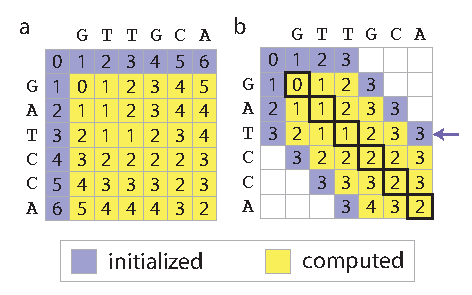
\includegraphics{NW.pdf}}
\caption{Needleman-Wunsch (NW) alignment. \textbf{a}
Alignment of GTTGCA and GATCCA using the NW alignment matrix. The
margins (purple) are initialized and the cells of the matrix (yellow)
are computed from left to right and from top to bottom by the following
dynamic programming algorithm. The value in each cell is computed from
the values of the neighboring top, left and top-left cells. Denoting
$a$, $b$ and $c$ these respective terms, the value in the cell of
coordinates $(i,j)$ is computed as $\min(a+1, b+1, c)$ if the $i$-th
letter from the first sequence is identical to the $j$-th letter from
the second, or $\min(a+1, b+1, c+1)$ if the letters are different. The
Levenshtein distance between the two sequences is found in the bottom
right cell. \textbf{b} Lower complexity algorithm to determine whether
GTTGCA and GATCCA are 2-neighbors. The values in purple cells are set
during initialization. The dynamic programming algorithm proceeds as
above, with the difference that it is interrupted if the value of a
diagonal cell (bold borders) is larger than 2. The values in purple
cells are not always the same as their equivalent in \textbf{a} (purple
arrow), but the values in the yellow cells are nevertheless identical.
The values of the white cells are never computed, which contributes to
making the algorithm less complex.}\label{fig:NW}
\end{figure}

In many instances, the only information of interest is to find out
whether the sequences are $d$-neighbors (separated by a distance less
than or equal to a threshold $d$).  In that case, the complexity then
reduces to $O(d \min(m,n))$ as described below \citep{ukkonen}. Instead
of initializing the margins of the matrix and computing all the terms,
the matrix is initialized as shown on Figure~\ref{fig:NW}b and only the
terms around the diagonal are computed. If the computation of a
diagonal term yields a value greater than $d$, the distance is known to
be greater than $d$ and the process is halted. Otherwise, the
bottom-right term indicates the actual distance between the sequences,
as in the NW algorithm.

This method can be used for inexact matching of sequences against a
reference set indexed as a prefix tree, also known as a trie
\citep{ukkonen}. The terms of the matrix are updated row-wise as a
depth-first search traverses the trie from the root, as illustrated
in Figure~\ref{fig:trie}. Every time a node is visited, the row
corresponding to its depth is recomputed. If the threshold value $d$
is exceeded for a diagonal term, the Levenshtein distance for all the
downstream sequences is also necessarily greater than $d$. Therefore,
no more hits are to be discovered in this path and the depth-first
search backtracks to the parent node. When the process halts, every
tail node (corresponding to a sequence of the database) on the path
of this search is a $d$-neighbor of the query. This method is
efficient because it eliminates large areas of the search space, and
because the NW alignment of the query with each prefix of the database
is computed only once.

\begin{figure}[!tpb]
\centerline{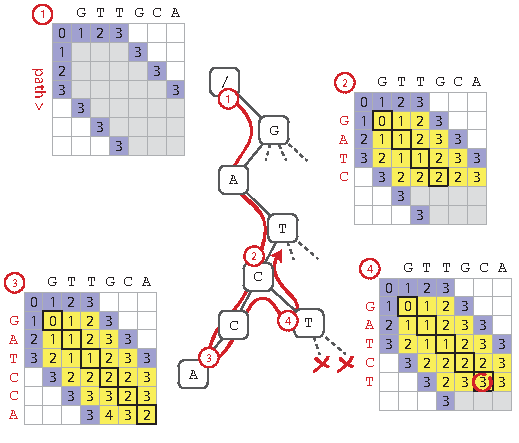
\includegraphics{trie.pdf}}
\caption{Trie query with NW alignment. Each sequence of the index is a
path in the trie. The query GTTGCA is written at the top of a NW matrix,
which is initialized as shown on Figure~\ref{fig:NW}b. The trie is
traversed by a depth-first search (red path) from the root. At each
depth, the node added to the path is written on the left of the NW
matrix and the row is computed. Checkpoints from 1 to 4 (circled red
numbers) show the state of the NW matrix as the search proceeds. The
node labeled 3 is a leaf and thus corresponds to a 2-neighbor of the
query. The search path then backtracks to the node labeled 2
and the last rows of the NW are erased. The search path then goes to
the node labeled 4, in which case the newly computed diagonal cell
exceeds the threshold (circled in red). Even if this node has children,
they are not visited (red crosses).}
\label{fig:trie}
\end{figure}


\subsection{The poucet search algorithm}
This strategy can be
further improved. Notice that if two consecutive queries share a prefix of length
$k$, the succession of computations up to the $k$-th row of the NW matrix will be exactly
the same in both queries. To take advantage of this property, the input sequences are
sorted alphabetically in order to maximize the prefix sharing. The main idea of the
algorithm is to store the computational intermediates in the nodes of the trie and
use them later to resume the computation in the next query. This way, the search can
start at depth $k$ whenever a query shares a prefix of such length with the previous
one.

However, storing the rows of the NW matrix in the nodes, as suggested by the
approach described in the previous section is not optimal. At depth equal to the
length of the shared prefix, say $k$, the terms on the right of the diagonal were
computed using characters that belong to the previous query. Since they also depend
on the terms computed at lower depth, the search cannot restart at depth $k$. This
issue is solved by storing in each node a combination of row and column terms that
form an angle shape, looking
like a horizontally flipped L character as shown on Figure~\ref{fig:poucet}. This way, the
computation intermediates stored in a node of depth $k$ depend only on the previous
characters of the query. Using this technique, the search can effectively restart
at a depth equal to the length of the shared prefix with the previous query, thereby
averting the need to recompute the first terms of the NW alignments.

In the fairy tale ``Le Petit Poucet'', the hero seeds white pebbles for his older
brothers to find their way home, which is reminiscent of the way queries pave
 the way for the next in this algorithm. We therefore called this search
algorithm ``poucet''.

\begin{figure}[!tpb]
\centerline{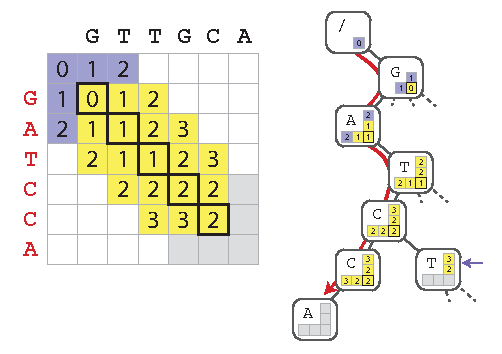
\includegraphics{poucet.pdf}}
\caption{Poucet search algorithm. The algorithm proceeds with the same principles
as shown on Figure~\ref{fig:trie} with the difference that the NW matrix is not
updated row-wise, but along horizontally flipped L shapes. As the depth-first
search proceeds, these values are stored in the nodes of the trie. Only the nodes
at the top contain initialized values; for the other nodes, the values at the
border are implicitly known to be 3. Since the values in the vertical part of
the flipped L are the same for every child of the same node, they are computed
only once (purple arrow). The values in the grey cells will be computed as the
search path (red) visits the node. Storing the intermediates in the nodes allows
the next query to restart at depth $k$ if it shares a common prefix of length
$k$ with the current query.}
\label{fig:poucet}
\end{figure}

\subsection{Lookup search}
If the Levenshtein distance of two sequences of length $L$ is
less than or equal to $\tau$, there must exist a perfect match between
them of at least $k =\lfloor L / (\tau+1)\rfloor$ nucleotides. We take
advantage of this property to build a lookup table containing all such
$k$-mers of the sequences already present in the trie. When a new
sequence is queried, all its subsequences are extracted and queried
against the lookup table. If none of the subsequences are found, the
minimum distance between the query and all the sequences in the trie
is necessarily greater than $\tau$, and the trie search can therefore
be omitted. This lookup is particulary useful for long query sequences
(see \ref{performance}), where $k$ is large and the probability
of an exact match between subsequences is small unless they are
actually related, i.e. they belong to the same cluster. With this
method, the absence of match is detected at the computational cost of
several table lookups, compared to the higher cost of measuring the
Levenshtein distance between long sequences.

In general, however, $L / (\tau+1)$ is not an integer. To deal
with this complication, we divide the query into $\tau+2$ subsequences.
The first $k+1$ are called \emph{words} and have a target length
$(L-\tau) / (\tau+1)$. The last subsequence is called \emph{tail} and has
length $\tau$. The length of the words is computed by integer
division, and the remainder $R$ is distributed equally among the last
$R$ words. As a result, the words have a length that differs by at
most 1, with an aggregated length equal to $L-\tau$.

Since two exact words at different positions in the sequence shall not
represent a lookup match, we store and query the words against $k+1$
distinct lookup tables. In order to allow insertions and deletions, 
the lookup search must also query shifted versions of each word. In
the worst matching case, only one word is found and the mismatches are
evenly distributed in the query sequence. In such case, the maximum 
number of cumulative insertions/deletions at the $i$-th word is
$i-1$. Hence, the $i$-th word has to be shifted and queried against
the lookup table $2(i-1)+1$ times to cover all the possible
cases. The last word will be queried $2\tau+1$ times, including
$\tau$ shifts on the right and $\tau$ shifts on the left. For the
latter shift we make use of the $\tau$ nucleotides stored in the
tail. The total number of lookups per sequence is $(\tau+1)^2$.

\subsection{Seek and construct}
To reduce the size of the search space, we use a dynamic ``seek and construct''
approach whereby queries are processed meanwhile the trie is built. In other
words, each sequence is matched against the trie before it is inserted. To
illustrate why the trie does not need to contain all the sequences upon query,
assume that two sequences A and B are $d$-neighbors. A is processed first. Since
B is not yet inserted, A yields no hit. It is then inserted in the trie. At the
time B is processed, A is a hit for the query and the match A-B is discovered.
This approach guarantees that every hit is discovered, while maintaining the
trie as ``thin'' as possible, thereby reducing the search time.
The whole matching process is summarized in the pseudocode shown in
Algorithms~\ref{alg:starcode} and \ref{alg:poucet}.

\begin{algorithm}
  \caption{Starcode algorithm}
  \label{alg:starcode}
  \begin{algorithmic}[1]
    \State \textbf{Define:} $\tau$
    \State \textbf{Variables:} $seed$, $start = 0$,
    $height$, $seq$, $trie$, $lastseq$, $k$
    \State \textbf{Containers:} $hits$, $pebbles$
    \State \textsc{read} sequence file
    \State $height \gets$ \textsc{determine} maximum sequence length
    \State \textsc{pad} sequences up to $height$
    \State \textsc{sort} sequences alphabetically
    \State $k \gets$ \textsc{compute} lookup word lengths
    \State $trie \gets$ \textsc{create} an empty trie of height $height$
    \State \textsc{insert} root node of $trie$ in $pebbles$ at depth 0
    \ForAll{sequences}
    \State $seq \gets$ \textsc{get} next sequence
    \If{at least one $k$-mer of $seq$ is in the lookup table}
    \State $seed \gets$ \textsc{length} of shared prefix
    between current and next sequence
    \State $start \gets$ \textsc{length} of shared prefix
    between $seq$ and $lastseq$
    \State \textsc{clear} hits
    \State \textsc{clear} $pebbles$ at depth $>start$
    \ForAll{$pebbles$ at depth $start$}
    \State $node \gets$ \textsc{get} next node from $pebbles$
    \State \textbf{call} \textsc{poucet}($seq$, $node$, $seed$,
    $hits$, $pebbles$)
    \EndFor
    \State \textsc{process} $hits$ and \textsc{link} matches to $seq$
    \State $lastseq \gets seq$
    \EndIf
    \State \textsc{insert} $seq$ path in $trie$
    \State \textsc{insert} $seq$ $k$-mers into the lookup table
    \EndFor
  \end{algorithmic}
\end{algorithm}

\begin{algorithm}
  \caption{Poucet search algorithm}
  \label{alg:poucet}
  \begin{algorithmic}[1]
    \Procedure{poucet}{$query$, $node$, $seed$, $hits$, $pebbles$}:
    \State \textsc{compute} $node$-specific column following NW
    \Comment{Fig.1}
    \ForAll{$child$ nodes in $node$}
    \State \textsc{compute} $child$-specific row following NW
    \Comment{Fig.1}
    \State \textsc{compute} center value using row and column \Comment{Fig.1}
    \If{center value $>\tau$} \Comment{Mismatches exceeded.}
    \State \textbf{continue} with next $child$
    \EndIf
    \If{$node$ depth = $height$} \Comment{Hit found.}
    \State \textsc{save} $node$ sequence in $hits$
    \State \textbf{continue} with next $child$
    \EndIf
    \If{$node$ depth $\leq seed$}
    \State \textsc{save} $node$ in $pebbles$ at current depth
    \EndIf
    \State \textbf{call} poucet($query$, $child$, $seed$, $hits$, $pebbles$)
    \EndFor
    \EndProcedure
  \end{algorithmic}
\end{algorithm}


\subsection{Parallelization}
To parallelize the search, queries are separated into contiguous blocks after
sorting. The matching algorithm proceeds in two phases. During the
first phase, an independent trie is created and filled with the
sequences of its associated block using the seek and construct process
described above. In the second phase, all the other blocks of
sequences are queried against but not inserted into each trie built in
the first phase. If the queries are segregated into $N$ blocks, the
first phase consists of $N$ seek and construct jobs, whereas the second
consists of $N(N-1)/2$ query jobs. Since the jobs show little
dependence on each other, the matching algorithm can be efficiently
parallelized provided $N$ is larger than the number of independent
threads.
\subsection{Clustering}
Starcode implements a multi-purpose clustering algorithm called ``sphere
clustering'' \citep{pmid23953119}, and a message passing algorithm
\citep{mackay} tailored for the task of clustering random barcodes. In
sphere clustering, barcodes are sorted by frequency of occurrence and
each barcode, starting from the most frequent, can claim its
$d$-neighbors that were not already claimed. 

In message passing clustering, read counts are distributed equally
among the closest neighbors of each barcode only if they are at least
5 times more frequent. The remaining sequences at the end of the
process are considered canonical, and their associated count is the
estimated cluster size. A barcode is assigned to a cluster if all its
read counts are eventually given to the corresponding canonical
barcode. The barcodes for which the read counts are split between
different canonical barcodes are not assigned to any cluster. The
reason for imposing a factor 5 or larger in order to transfer the read
counts is that barcodes with similar frequencies are not likely
derived from each other through sequencing errors. More likely they
are either unrelated, or they both derive from another more abundant
barcode. 

\end{methods}

\section{Results}

\subsection{Performance}
\label{performance}
We measured basic performance and scalability metrics of starcode on a
dataset of pseudo random sequences (Figure~\ref{fig:perf}). The standard
configuration consists of a set of 1,000,000 sequences of length 40 running
on 1 thread and with a maximum Levenshtein distance of 3. To test the
scalability as a function of a single parameter, only the parameter under
study was modified whereas the others were kept constant. 

Figure~\ref{fig:perf}a shows the running time of starcode as a
function of the number of input sequences $n$. In double logarithmic scale
the trend is a straight line with slope 1.7, which suggests that the
running time complexity of starcode is approximately $O(n^{1.7})$.
Figure~\ref{fig:perf}b shows that the running time grows exponentially
as a function of the maximum Levenshtein distance used for clustering.
This is a common feature of exact algorithms based on trie search. As
this parameter increases, the poucet search bails out at a greater
average depth in a trie that fans out exponentially.
As a function of the sequence length, the running time first increases 
but then plummets and stays low (Figure~\ref{fig:perf}c).
Beyond a certain length, the lookup search algorithm starts to be
efficient, and most of the queries are resolved without the need for
trie-search.
Finally, we show the scalability of starcode with increasing
number of threads in Figure~\ref{fig:perf}d. The search algorithm is fully
parallel and the relative performance increases linearly up to 8 threads.
The bending observed thereafter has two sources. The first is 
that the input reading and clustering steps are brief but not parallel,
the second is that there is insufficient memory bandwidth to satisfy
the increased demand of memory accesses due to hardware limitations.


\begin{figure}[!tpb]%figurex
\centerline{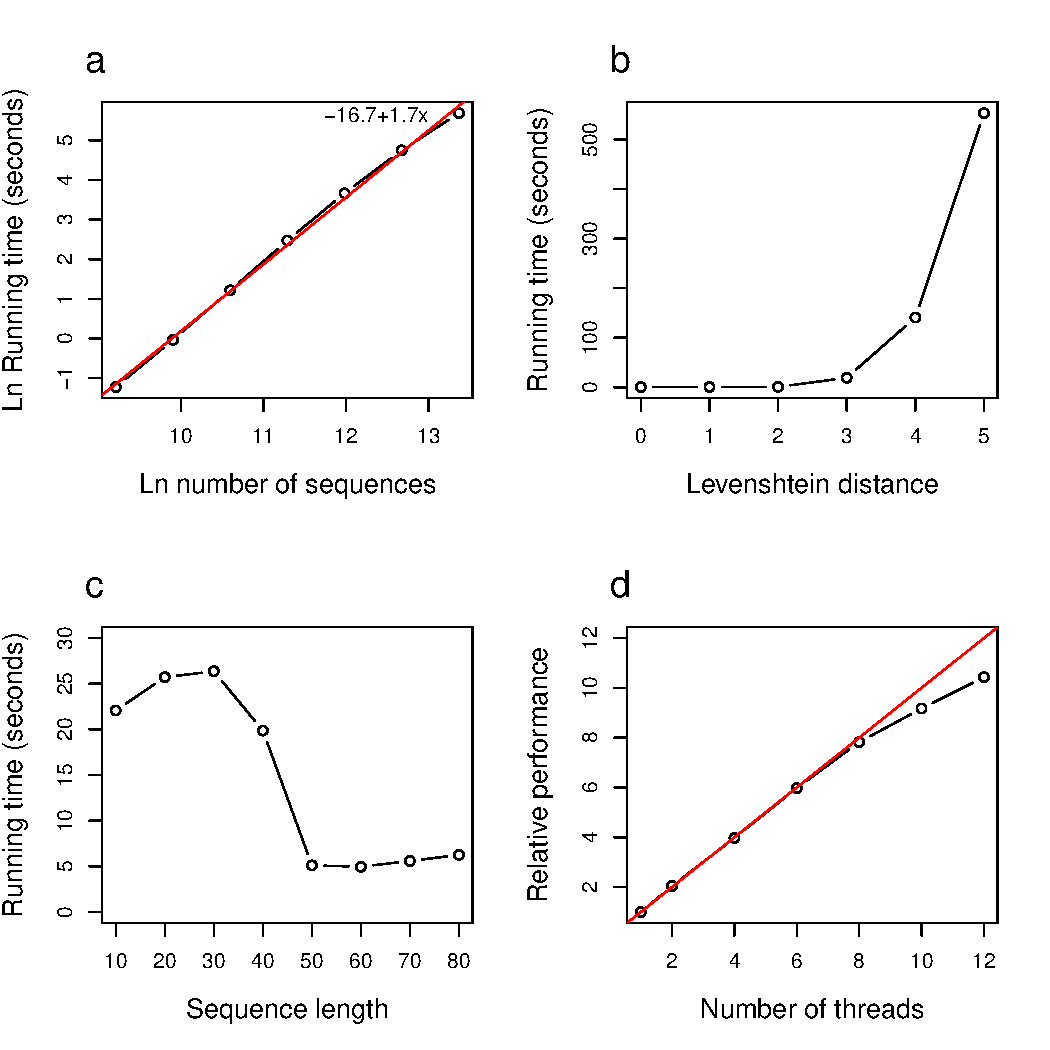
\includegraphics[scale=0.47]{scalability.pdf}}
\caption{Scalability. a. Logarithm of the running time versus the
logarithm of the number of sequences to be clustered. b. Running time as
a function of the clustering distance. c. Running time versus length of
the input sequences. d. Relative performance increase for different number
of parallel threads. 
}\label{fig:perf}
\end{figure}


\subsection{Benchmark against sequence clustering algorithms}
Sequence clustering is routinely used to curate databases of non
redundant nucleotide or protein sequences. We benchmarked starcode
against the two popular sequence clustering algorithms CD-HIT
\citep{pmid23060610} and USEARCH \citep{pmid20709691}.

We generated 1 million random 40-mers duplicated 47 times. For each
40-mer, we also inserted 3 additional mutant sequences to the pool
by sampling again 3 nucleotides at random positions. The probability
that such a mutant sequence is within a distance 3 of any other
40-mer is of the order of $10^{-12}$ and can be neglected. Each
cluster thus consists of 50 sequences, of which 3 have a Levenshtein
distance 3 from the canonical representant (referred to as the centroid
in clustering terms).

All software were set to run on a 6-core single-processor Intel Xeon
E5-2620 system with 48~GB of DDR3-RAM at 1333~Mhz.
Using 12 threads, starcode clustered the shuffled 50 million sequences
in 5 minutes and 3 seconds without a single error (the output
consisted of 1 million clusters of size 50). There is no obvious
way to compare exact algorithms with heuristic algorithms such as
CD-HIT and USEARCH. We decided to allocate the heuristics 6 minutes
on the same dataset (20\% additional time) and use the
parameters giving the best accurary under this constraint.
However, we could not find a combination of
parameters such that either of them could terminate in less than
6 minutes. To simplify the task, we extracted the unique sequences
from the input file, bringing the number down to 4,000,000 and followed
the same rationale. We could not find any set of parameters such
that USEARCH could process this input in less than 6 minutes
(because of poor multi-threading performance), but CD-HIT could
perform the task when run as shown in Table~\ref{tab:params1}.
In such conditions, it identified 2,798,656 clusters, indicating that
the clustering was not nearly complete.

\begin{table}[h]
\centering
\caption{Software execution parameters (benchmark 1)}
\resizebox{\columnwidth}{!}{
\begin{tabular}{|l|l|}
    \hline
    starcode & \texttt{-d3 -t12 -s}\\ \hline
    CD-HIT 4.6.1 & \texttt{cd-hit-est -n 7 -c .925 -T 12 -M 0 -r 0 -A 40}\\ \hline
\end{tabular}
}
\label{tab:params1}
\end{table}

We next benchmarked starcode on the biological dataset used by
\cite{pmid23060610}. Because USEARCH imposes a memory limit on the
size of the input file, we clustered the forward reads on 95\%
identity from one lane only (reference ERR011089), adding up to
4,189,859 reads, each 75 nucleotides long. Using 12 threads, starcode
identified 4,111,111 clusters in 6 minute 19 seconds. Allocating up to
7 minutes 30 seconds to CD-HIT and USEARCH, we selected the parameters
giving highest accuracy. In such conditions (see Table~\ref{tab:params2})
CD-HIT identified 4,126,352 clusters while USEARCH could not be run in
the allocated time. These results indicate that starcode achieves good
performance on clustering high throughput sequencing reads.

\begin{table}[h]
\centering
\caption{Software execution parameters (benchmark 2)}
\resizebox{\columnwidth}{!}{
\begin{tabular}{|l|l|}
    \hline
    starcode & \texttt{-d4 -t12 -s}\\ \hline
    CD-HIT 4.6.1 & \texttt{cd-hit-est -n 8 -c .95 -T 12 -M 0 -r 0 -A 75}\\ \hline
\end{tabular}
}
\label{tab:params2}
\end{table}


\begin{figure}[!tpb]
\centerline{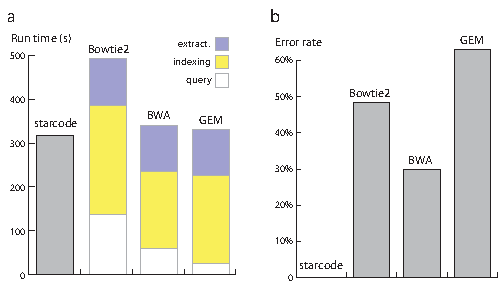
\includegraphics{benchmark.pdf}}
\caption{Benchmark of starcode against short read mappers.
\textbf{a} Running time compared to Bowtie2, BWA and GEM on the
dataset described in the text. The running time is decomposed as
extraction of unique sequences (purple), Burrows-Wheeler indexing
(yellow) and query proper (white). The extraction was performed with
the Linux \texttt{sort} command, so the time is the same in every
case. \textbf{d} Error rate compared to Bowtie2, BWA and GEM,
expressed as the proportion of matches with a single hit. This is an
underestimate of the true error rate.}
\label{fig:benchmark}
\end{figure}


\subsection{Benchmark against short read mappers}
A potential strategy to cluster short sequences is to use
Burrows-Wheeler transform-based short read mappers to match a set of
sequences against itself. Once matches are available, several community
detection algorithms can be used to identify the clusters. We 
benchmarked starcode against the short read mappers Bowtie2
\citep{pmid22388286}, BWA \citep{pmid19451168} and GEM
\citep{pmid23103880}. Short read mappers do not perform clustering, so
we only evaluated their performance on the matching problem.

For this test, we used the first dataset described above, in which
every sequence has at least 2 distinct matches at a distance 3 (mutant
sequences from the same cluster may be at a distance up to 6 from each
other, but their distance to the centroid is always 3). This means that
we can use matches with a single hit (every read trivially matches
itself) as a lower bound on the inaccuracy. We used the 4,000,000 unique
40-mers to build an index that was later queried with the same 40-mers
using parameters shown in Table~\ref{tab:srm}.

\begin{table}[h]
\centering
\caption{Software execution parameters (benchmark 3)}
\resizebox{\columnwidth}{!}{
\begin{tabular}{|l|l|}
    \hline
    Bowtie2 indexer & \texttt{bowtie2-build --quiet}\\ \hline
    Bowtie2 2.1.0 & \texttt{-f -a -p 12 --no-hd --very-sensitive}\\ \hline
    BWA indexer & \texttt{bwa index -a is}\\ \hline
    BWA 0.7.9a & \texttt{mem -t 12 -a -k1 -B0} \\ \hline
    GEM indexer & \texttt{gem-indexer -T 12} \\ \hline
    GEM 1.423 & \texttt{-e3 -s4 -T12 --granularity 100000}\\ \hline
\end{tabular}
}
\label{tab:srm}
\end{table}

Figure~\ref{fig:benchmark}a shows the running time of starcode along
with the decomposition of the running time for the three mappers. Note
that the time to extract unique sequences is always the same because
we used the Linux \texttt{sort -u} command in every case. The running
time of starcode is slightly lower than short read mappers when all
steps ares taken into account. Figure~\ref{fig:benchmark}b shows the
lower bound on the error rate, as estimated by the proportion of single
hits. BWA was found to be the most accurate aligner with a lower bound
of 31\% sequences with a single match. This measure is an underestimate
of the true error rate, but given that starcode is an exact algorithm,
a more accurate measure is not necessary: starcode can compete with the
short read aligners on the matching problem, and it provides a precision
that none of the other tools can offer.

\subsection{Clustering TRIP barcodes}
In the course of setting up the TRIP technology in our laboratory
\citep{pmid23953119}, we realized the need to develop efficient
algorithms to cluster similar sequences. Briefly, the principle of TRIP
(Thousands of Reporters Integrated in Parallel) is to tag reporter
transcripts with random barcodes and measure the abundance of barcodes
in the RNA as a proxy for gene expression. There is no reference to
match aberrant barcodes against, because the tagging sequences are
unknown. Instead, barcodes are matched against each other and clustered
by similarity to infer canonical sequences.

We tested the efficiency of starcode on the TRIP dataset from
\cite{pmid23953119}. In the experiment labeled mPGKA, we identified
24.1 million (91\%) barcode-containing reads out of 26.6 million,
consisting of approximately 223,000 and 220,000 unique barcode sequences
for PCR replicates 1 and 2, respectively. Following the authors, we kept
only the barcodes with at least 5 counts and performed clustering as
described: ``First we sorted barcodes according to their counts. Then,
for each barcode (starting from the most frequent one), we identified
and removed all its mutant versions, defined as barcodes within a Hamming
distance of 2.'' We implemented this method, here on referred to as the
``sequential algorithm'' with the function call
\texttt{stringDist(method='lv', maxDist=2)} from R the package
\texttt{stringDist} \citep{R}.  When replacing the Hamming distance by
the Levenshtein
distance, starcode produced exactly the same output as the sequential
algorithm. The running time of starcode averaged over the replicates was
2.90 seconds, \textit{versus} more than 3 minutes 40 seconds, which
represents a 75-fold speedup.

The performance of the sequential algorithm relies on the arbitrary
exclusion of reads with less than 5 counts, the main purpose of which
is to reduce the computational burden. When all barcodes were kept,
the average running time of starcode was 10.27 seconds, \textit{versus}
$>$ 6 hours for the sequential algorithm. Using the Hamming distance,
as the authors originally suggested, decreased the average running time
of the sequential algorithm to about 3 hours and 30 minutes (and
the output differed from that of starcode). Note that in all the cases
mentioned above, starcode was run with a single core to compare the
algorithms based on similar computer resources. In conclusion, the
barcode clustering problem can be simplified by various tricks, but
starcode brings down the running time to nearly instantaneous, and
thereby obviates the need for such arbitrary heuristics.

\subsection{Identifying enriched sequence motifs}
Sequence motifs are thought to play an important role in DNA metabolism.
Key regulators, such as transcription factors, nucleosomes and non
coding RNAs have sequence preferences targeting them to the sites where
they act. Identifying those sequences is a way to pinpoint the
regulators and the mechanisms they are involved in. However, the
sequence motifs are not strictly identical at different sites, hence
they are better identified by inexact matching. This problem becomes
computationally difficult for long motifs (above 12-13 nucleotides)
because of the combinatorial scaling. But as motifs become longer, the
problem of identifying abundant inexact matches becomes similar to
barcode clustering. We reasoned that starcode could also be used for
the task of identifying biologically meaningful sequence motifs.

We set up a test based on the meningitis-causing agent
\textit{Neisseria meningitidis}. The genome of this bacterium is
interspersed with a frequent 12 bp sequence known as DNA uptake
sequence \citep{pmid10673000}. We extracted the 12-mers from both
orientations of �the 2.19 Mb genome, yielding 4.39 million 12-mers,
consisting of 2.77 million unique sequences. Clustering the 12-mers
with starcode within a Levenshtein distance of 2 took less than 45
seconds with 12 threads. We identified the known DNA uptake sequence
of \textit{Neisseria meningitidis} (ATGCCGTCTGAA) as the most abundant
12-mer, with 1466 exact and 2096 inexact hits. This result testifies
to the fact that starcode can be used to identify biologically
relevant motifs in bacterial genomes.

To test starcode on another application, we used the RNA-protein
interaction data produced by RNAcompete \citep{pmid19561594}. The
mammalian splicing factor SRSF1 is known to bind RNA GA-rich motifs,
but there is some disagreement about the motif that it recognizes
\citep{pmid23562324}. For each replicate of the human SRSF1 in the
RNAcompete dataset, we replaced the microarray signals by their rank
and extracted the 10-mers from the microarray probes. The 10-mers were
given a score equal to the rank of the probe they belong, and enriched
motifs were found using the sphere clustering of starcode with maximum
Levenshtein distance 2. The score of the most enriched 10-mer is thus
the sum of the ranks of all 10-mers within this distance. Clustering
the 6.3 million extracted 10-mers with 12 threads took about 20 seconds
for each replicate.  The most enriched 10-mers were AGGACACGGA,
AGGACACGGA, AGGACGGAGG, AGGACGGAGG, AGGACACGGA and AGGATACAGG. Except
for the last replicate, the motifs consist of AGGAC and GGA, with a
spacer of variable length. This suggests that the binding of SRSF1 to
RNA may involve a spacer sequence, which would explain the disagreement
between the motifs derived from 6-mers or 7-mers.

\section{Discussion and conclusion}
Through the parallel poucet search algorithm, starcode implements an
exact sequence clustering algorithm that can be faster than popular
heuristics. By design, starcode is tailored to process high throughput
sequencing data on multi-core platforms. Our benchmark shows that
starcode achieves perfect clustering on short random sequences in less
time than what is considered acceptable for heuristic searches. We also
show that starcode outperforms next generation read mappers in this
context. The software tools used for this benchmark are usually not
used for barcode or random sequence clustering. In this respect,
starcode fills a need arising from the development of barcoding
technologies.

The speed of starcode also makes it useful for other clustering
tasks, such as identifying enriched motifs in microbial genomes and
in experimental data. Here we have given two examples of such
applications. In the first, we recover a known enriched 12-mer in the
genome of \textit{Neisseria meningitidis}. In the second, we recover
the motif of the human RNA binding protein SRSF1 and notice that it
seems to consist of two halves separated by a linker. This hypothesis
is consistent with the fact that SRSF1 binds RNA through two
consecutive RNA Recognition Motifs (RRM) that are known to bind
3-4 nucleotides in a row\citep{pmid23253355}. The Levenshtein distance,
which incorporates insertions and deletions is more likely to capture
bi-partite binding motifs than position weight matrix representations.
The use of a clustering method to tackle this problem is unusual, but it 
it illustrates the potential advantages of distance-based approaches.

The current version of starcode has been primarily optimized for speed.
The memory footprint depends on the number of sequences to cluster
(because the sequences of the input set are loaded in memory as a set of
of tries) and on the mean number of matches per sequence. Every match is
stored in memory until the clustering phase, which may represent a large
overhead if the dataset is dense. As counterintuitive as it may seem,
long queries will usually impose a lower memory footprint because the
matches between the sequences are more sparse. We have shown that the
running time will also be shorter thanks to the lookup table
search (Figure~\ref{fig:perf}c).

Perhaps the most surprising element of this study is that an exact
algorithm can compete with extremely fast heuristics. This will no
longer be true when clustering divergent sequences because the Levenshtein
distance will have to be increased, leading to exponentially longer
running times (Figure~\ref{fig:perf}b). However, for the imporant
practical case that the divergence is driven by sequencing errors,
starcode illustrates that there is still room for algorithmic innovations
that can outperform heuristics. The idea of the poucet search seems
simple in retrospect, yet it is a powerful way to tap into the data
structuration provided by string sorting. This principle could find some
applications in algorithms used in various fields.


%%%%%%%%%%%%%%%%%%%%%%%%%%%%%%%%%%%%%%%%%%%%%%%%%%%%%%%%%%%%%%%%%%%%%%%%%%%%%%%%%%%%%
%
%     please remove the " % " symbol from \centerline{\includegraphics{fig01.eps}}
%     as it may ignore the figures.
%
%%%%%%%%%%%%%%%%%%%%%%%%%%%%%%%%%%%%%%%%%%%%%%%%%%%%%%%%%%%%%%%%%%%%%%%%%%%%%%%%%%%%%%


\section*{Acknowledgement}
We would like to thank Maria Chatzou for her precious feedback on the
preliminary version of this manuscript.

\paragraph{Funding\textcolon}
The research leading to these results has received funding from the
Government of Catalonia (Dept. of Economy and Knowledge) and the Spanish
Ministry of Economy and Competitiveness (Centro de Excelencia Severo Ochoa
2013-2017' (SEV-2012-0208). P.C. fellowship is partly financed by the
Spanish Ministry of Economy and Competitiveness (State Training Subprogram:
predoctoral fellowships for the training of PhD students (FPI) 2013).

\bibliographystyle{natbib}
%\bibliographystyle{achemnat}
%\bibliographystyle{plainnat}
%\bibliographystyle{abbrv}
%\bibliographystyle{bioinformatics}
%
%\bibliographystyle{plain}
%
\bibliography{document}


%\begin{thebibliography}{}
%\end{thebibliography}
\end{document}
